\usepackage{setspace}

\clearpage
\section{Dynamic Huffman Coder and Decoder}

\begin{refsection}

\begin{tcolorbox}	
\begin{tabular}{p{2.75cm} p{0.2cm} p{10.5cm}} 	
\textbf{Students Name}  &:& Cristiano Ferreira Gon\c{c}alves (10/06/2018 - 29/06/2018) \\
\textbf{Starting Date} &:& June 10, 2018\\
\textbf{Goal}          &:& Huffman coding and decoding of text.
\end{tabular}
\end{tcolorbox}

Dynamic Huffman code can compress text very effectively for medium-long texts without previous knowledge of the characters probability.

\subsection{Code Analysis}

\hspace{5mm} This code is stored and based on a Huffman tree, for example as the one of Figure \ref{fig:hufftree}. This tree stores in its leafs $($bottom nodes$)$ the characters. The code is attributed by the path from the root to each character, for each level of the tree is attributed an '1' if the path follows through the right soon or a '0' if it follows left.

\begin{figure}[H]
	\centering
	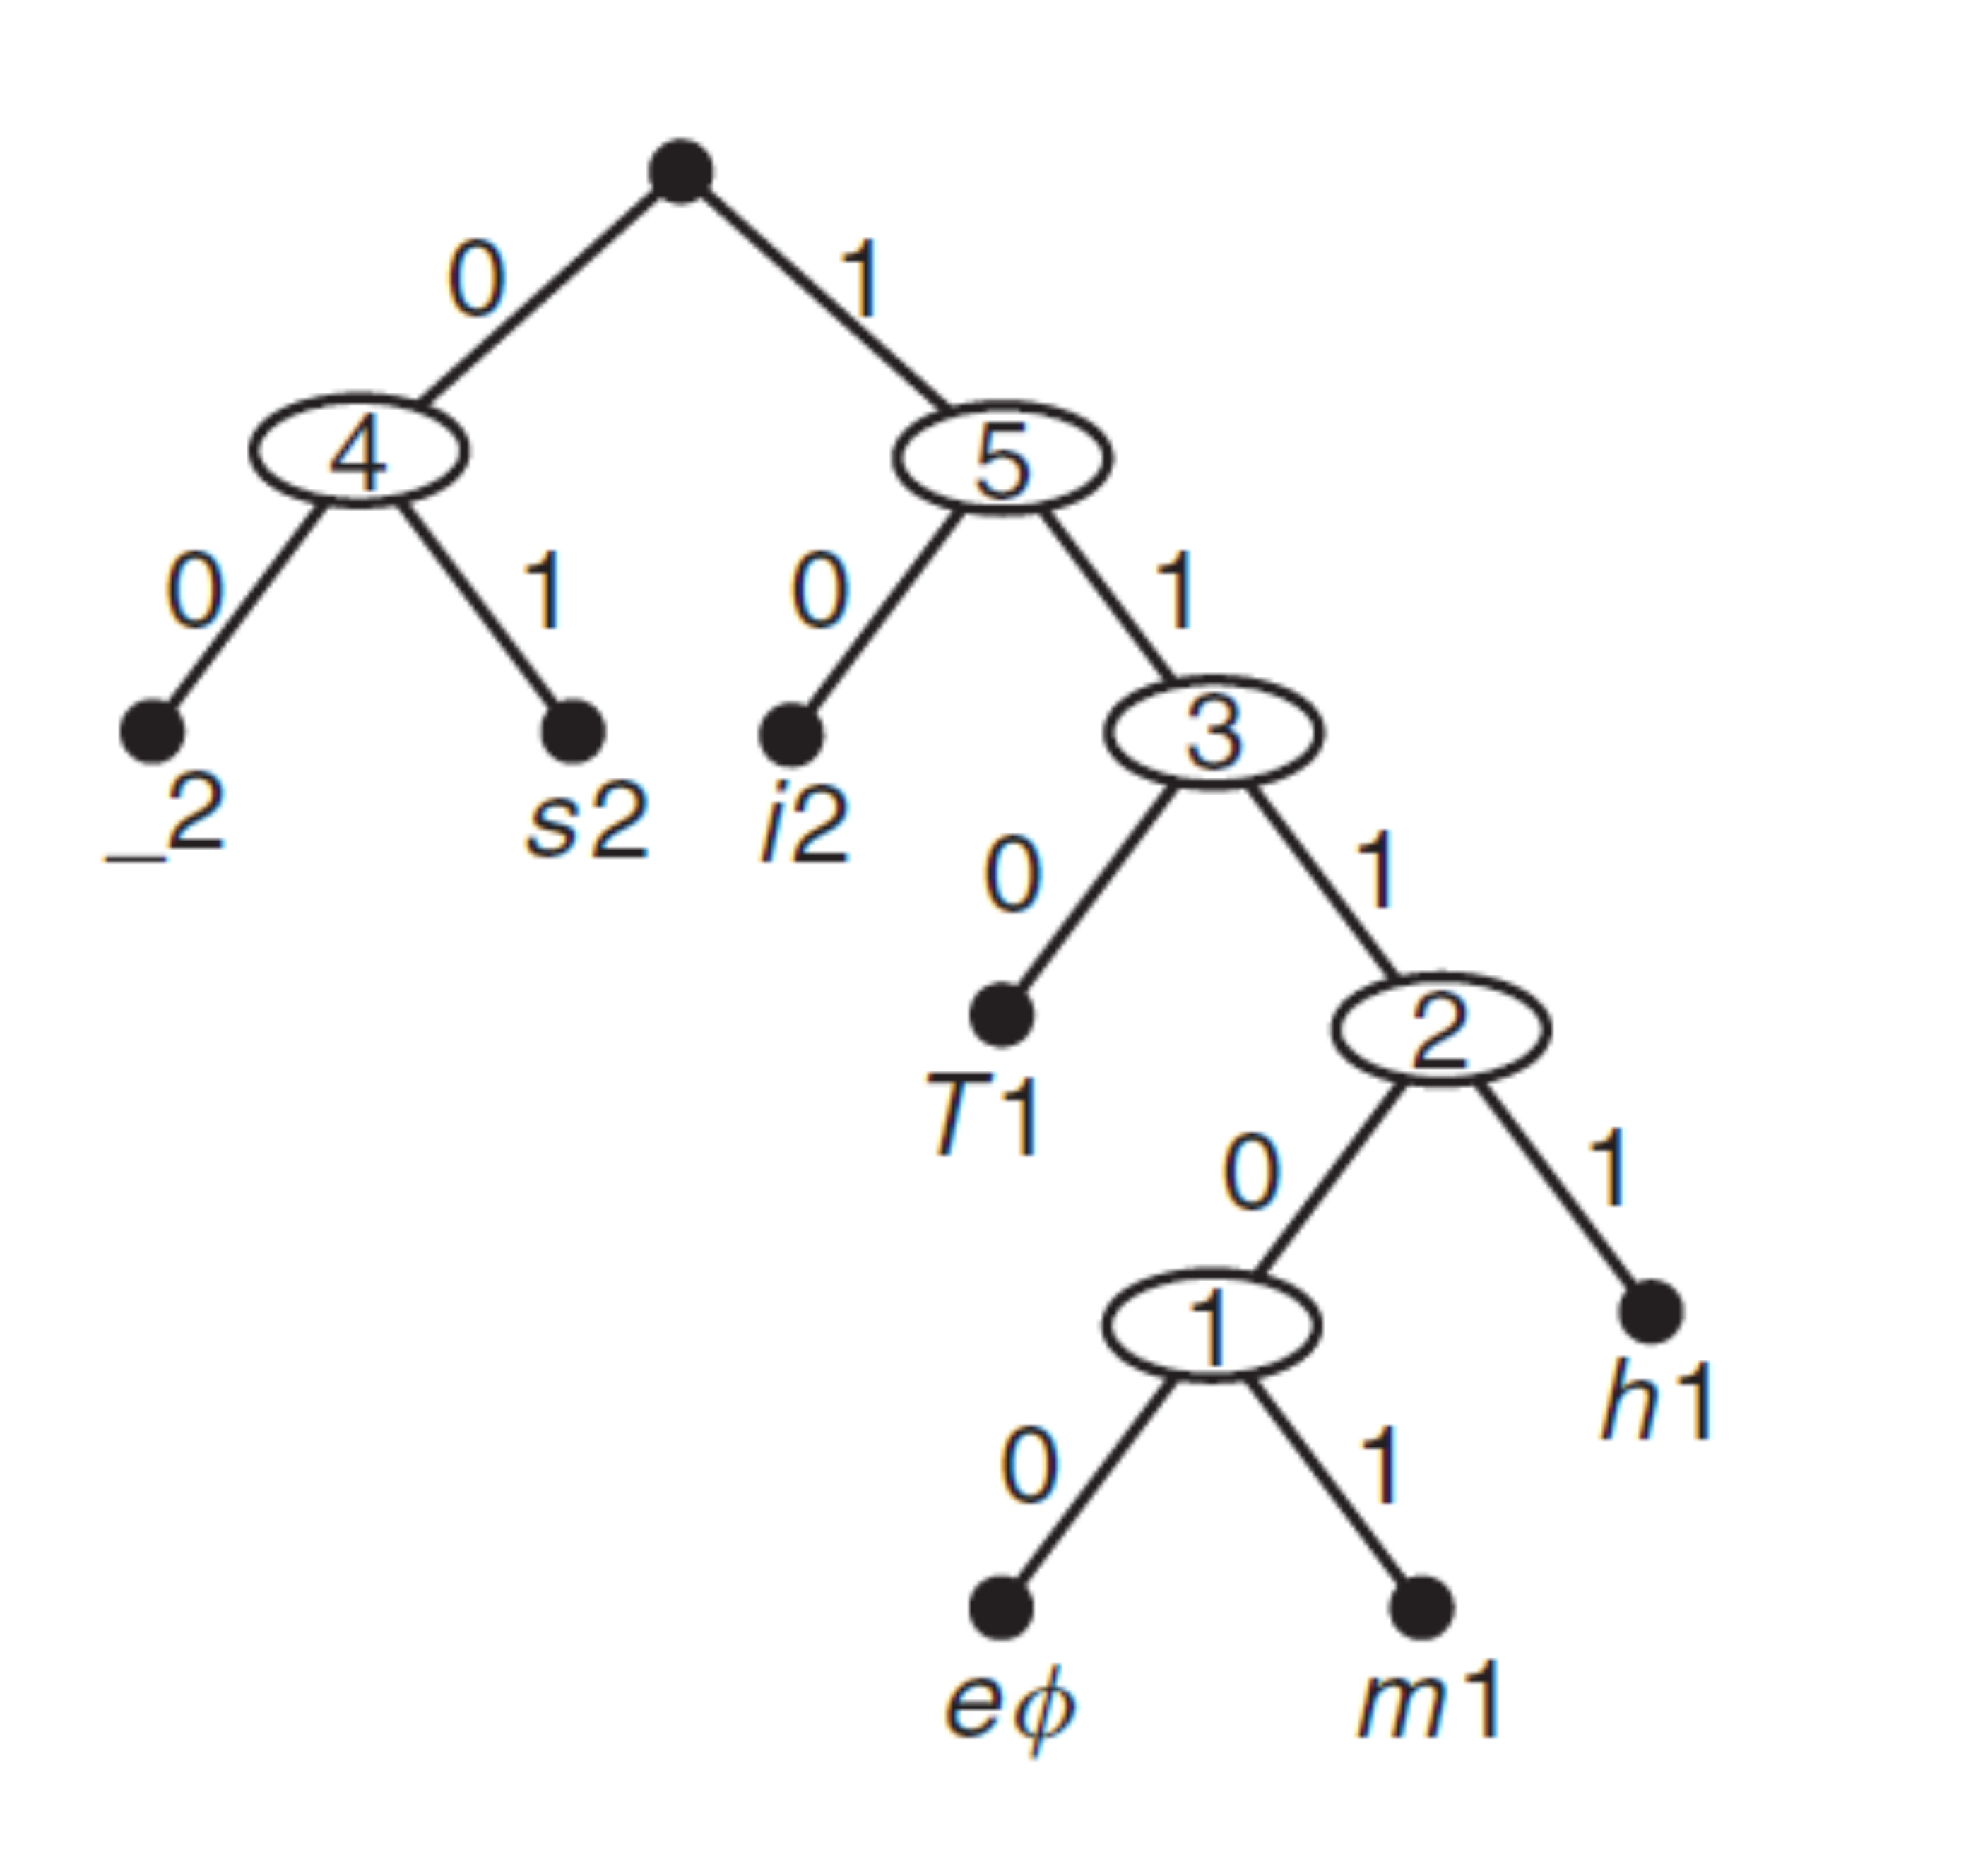
\includegraphics[width=0.5\textwidth,height=7cm]{./sdf/eit_64926_dynHuff_CoderDecoder/figures/HuffTree.png}
	\caption{Ordered Huffman tree example (figure from \cite{DigComm}).}\label{fig:hufftree}
\end{figure}

For each of the nodes 4 variables are stored:
\begin{itemize}
	\item The character stored in the node;
	\item The frequency of the character $($number of times it appeared$)$;
	\item The pointer to the right soon node;
	\item The pointer to the left soon node.
\end{itemize}
\vspace{2cm}

When a new character is received two cases can happen:
\begin{itemize}
\item The character already exists and its frequency is incremented by one.
\item The character do not exists on the tree and a new node is added for it.
\end{itemize}

For the last case, the node is added as right soon of the previous empty node and the new empty node becomes the left soon of the previous empty node.\\
After each modification the tree is reordered so its leafs from left to right and bottom-up are in ascending order of frequency. For the case described in Figure \ref{fig:hufftree}, it would be: 
\[ e\emptyset \quad m1 \quad 1 \quad h1 \quad T1 \quad 2 \quad \_2 \quad s2 \quad i2 \quad 3 \quad 4 \quad 5 \]
\hspace{5mm} The previous sequence is correctly ordered in terms of frequency. However for the example of Figure \ref{fig:hufftree2} the order would be:
\[ e\emptyset \quad \_2 \quad 2 \quad T1 \quad h1 \quad s2 \quad i2 \quad 3 \quad 3 \quad 5 \]

\begin{figure}[H]
	\centering
	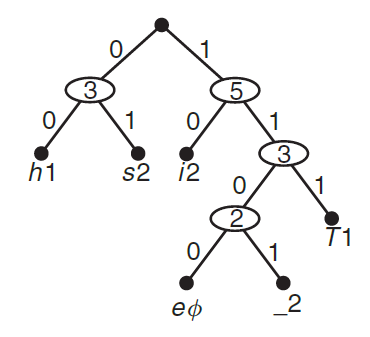
\includegraphics[width=0.5\textwidth,height=7cm]{./sdf/eit_64926_dynHuff_CoderDecoder/figures/HuffTree2.png}
	\caption{Not ordered Huffman tree example (figure from \cite{DigComm}).}\label{fig:hufftree2}
\end{figure}


For this case the nodes \_2 and h1 should be swapped. This swap should be done between the first higher node $($\_2 instead of 2$)$ and the last lower one $($h1 instead of T1$)$ so the sub-tree becomes always ordered and the tree gets fully ordered faster. 

\subsection{Practical Test}

\hspace{5mm} The algorithm has been implemented and the respective program used to encode the following text:\\
{\tiny "Nowadays, the power amplifier (PA) design paradigm is changing. Modern wireless networks push for PAs bandwidth, higher efficiencies and improved linearity requiring the use of more complex architectures [1][2]. Therefore, although the PA design methodology based on load-pull and S-parameter measurements obtained good results in the past [3], it is now very difficult to achieve the required figures of merit maintaining these design methodologies. This being the case, the use of CAD programs with accurate nonlinear models becomes of paramount importance. Such models have been intensively described in literature [4][5], and are particularly interesting in the case of high frequency designs, mainly for the future mm-wave 5G networks, since at these frequencies the load-pull measurements are much harder to perform and the required equipment is very specific and expensive. The problem with this approach is that the obtained PA performance is strongly dependent on the accuracy of the used device models, which is strongly correlated with the quality of the measurements performed during the nonlinear model extraction [6].
Gallium Nitride (GaN) High Electron Mobility Transistors (HEMTs) are predominantly adopted on these new mm-wave state-of-art PAs due to their advantages in terms of power density, cut-off frequency and high thermal conductivity. However, these devices are still affected by many frequency dispersive phenomena as thermal and trapping effects [7]-[9]. These problems cause a substantial discrepancy between their static and dynamic characteristics. Thus, in order to properly model their behavior isodynamic measurements are necessary, which leads to more sophisticated measurement setups. 
There are two main approaches to characterize these new devices: (i) Continuous wave (CW) excitations to cover the entire I/V plane [10], which implies a complicated curve-fitting process to simultaneously extract the resistive and reactive components of the device. (ii) Pulsed I/V and S-parameter measurements [11][12], for which a system that allows the generation of very fast, high-power and arbitrary waveform pulses is necessary. In these last ones, the capability to generate arbitrary bias signals is of remarkable importance, because it allows to generate specific waveforms that are necessary to guarantee isothermal measurements and avoid dispersive phenomena [11]. There are already pulsed measurements systems able to generate 100 V and 7 A pulses with 600 ns settling time [13]-[15], and some modern pulsers that can handle 5000 W or even higher instantaneous power [16][17]. However, they are very expensive and unable to generate the necessary waveforms.
Compared to the available ones, this paper presents a cost effective and more versatile measurement system, which allows the use of arbitrary waveform signals. This makes possible to obtain accurate and isodynamic pulsed measurements. Thus, the main contributions of this paper are the power head and respective characterization signal waveform design. To test the implemented system a 15 W GaN device from Wolfspeed was measured and shown to be mainly affected by drain lag and temperature effects. The second part of this paper is dedicated to the measurement setup and pulser implementation. The third section will be devoted to the waveform design. Lastly, in the fourth section, the measurements will be compared with I/V curves obtained from the integration of the small signal transcondutance $($g\textsubscript{m} $)$ and output conductance $($g\textsubscript{ds}$)$. The good agreement obtained between all the sets of curves attests its isodynamic behavior."}\\

This text has been encoded without any error in 60\% of its original size, as shown in Figure \ref{fig:encodedtext}. The total size decreased from 3.6KB to 2.2KB.

\begin{figure}[H]
	\centering
	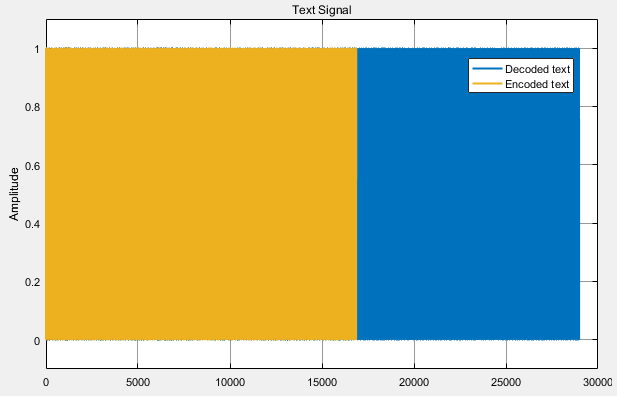
\includegraphics[width=0.7\textwidth,height=7cm]{./sdf/eit_64926_dynHuff_CoderDecoder/figures/textSignals.png}
	\caption{Matlab visualization of the encoded and decoded signals of the example text.}\label{fig:encodedtext}
\end{figure}

% Bibliography
\newpage
\clearpage
\printbibliography[heading=subbibliography]
\end{refsection}
\addcontentsline{toc}{subsection}{Bibliography}
\cleardoublepage